\documentclass[11pt, a4paper]{article}

% --- UNIVERSAL PREAMBLE BLOCK ---
\usepackage[a4paper, top=2.5cm, bottom=2.5cm, left=2cm, right=2cm]{geometry}

% Graphics and Drawing
\usepackage{tikz}
\usetikzlibrary{arrows.meta, calc, positioning, patterns, decorations.pathreplacing, 3d}

\usepackage{amsmath}
\usepackage{xcolor}

% --- UNIVERSITY OF SOUTH CAROLINA MARKETING TOOLBOX COLOR DEFINITIONS ---
% Primary Colors
\definecolor{UofSCGarnet}{RGB}{115, 0, 10}
\definecolor{UofSCBlack}{RGB}{0, 0, 0}
\definecolor{UofSCWhite}{RGB}{255, 255, 255}

% Neutral Colors
\definecolor{UofSC90Black}{RGB}{54, 54, 54}
\definecolor{UofSC70Black}{RGB}{92, 92, 92}
\definecolor{UofSC50Black}{RGB}{162, 162, 162}
\definecolor{UofSC30Black}{RGB}{199, 199, 199}
\definecolor{UofSC10Black}{RGB}{235, 235, 235}
\definecolor{UofSCWarmGrey}{RGB}{103, 97, 86}
\definecolor{UofSCSandstorm}{RGB}{255, 242, 227}

% Accent Colors
\definecolor{UofSCRose}{RGB}{204, 46, 64}
\definecolor{UofSCAtlantic}{RGB}{70, 106, 159}
\definecolor{UofSCCongaree}{RGB}{31, 65, 77}
\definecolor{UofSCHorseshoe}{RGB}{101, 120, 11}
\definecolor{UofSCGrass}{RGB}{206, 211, 24}
\definecolor{UofSCHoneycomb}{RGB}{164, 145, 55}

% Special Use Colors
\definecolor{UofSCDarkGarnet}{RGB}{87, 0, 8}
\definecolor{UofSCAzalea}{RGB}{132, 66, 71}

\title{Aeroelastic Wing Problem Diagram}
\date{}

\begin{document}

\begin{figure}[htbp]
    \centering
    % --- DIAGRAM 1: 3D Isometric View of the Wing ---
    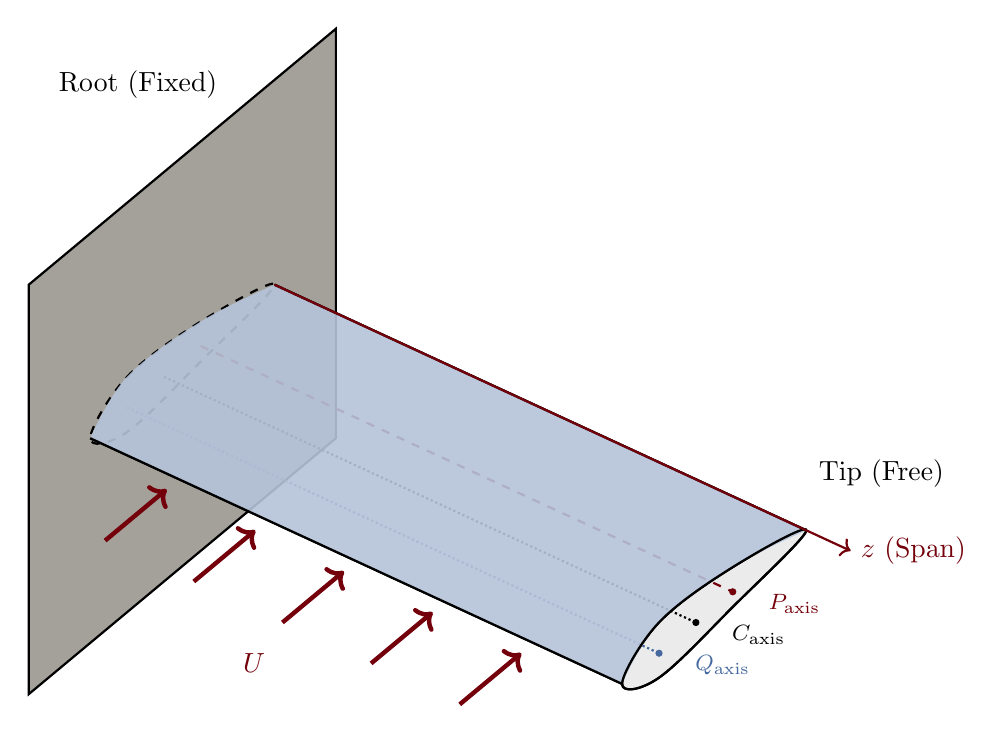
\begin{tikzpicture}[x={(0.866cm,-0.4cm)}, y={(0.6cm,0.5cm)}, z={(0cm,1cm)}, scale=1.3]

        % Constants
        \def\span{6}   % Length along z axis (visual span)
        \def\chord{3}  % Chord length
        
        % Wall (Root)
        \fill[UofSCWarmGrey!60] (0, -1, -2) -- (0, \chord+1, -2) -- (0, \chord+1, 2) -- (0, -1, 2) -- cycle;
        \draw[thick] (0, -1, -2) -- (0, \chord+1, -2) -- (0, \chord+1, 2) -- (0, -1, 2) -- cycle;


        % Define Airfoil shape command
        % #1: x-offset (spanwise position)
        \newcommand{\drawAirfoil}[1]{
            plot [smooth cycle, tension=0.6] coordinates {
                (#1, 0, 0)           % Leading Edge
                (#1, 0.2*\chord, 0.1*\chord) % Upper surface 1
                (#1, 0.6*\chord, 0.08*\chord) % Upper surface 2
                (#1, \chord, 0)      % Trailing Edge
                (#1, 0.6*\chord, -0.05*\chord)% Lower surface 2
                (#1, 0.2*\chord, -0.08*\chord)% Lower surface 1
            }
        }

        % Draw the Wing Surface (Extrusion)
        % We draw the tip profile, then lines connecting to root (hidden by wall, but we start at 0)
        
        % 1. Bottom Surface Lines (Root to Tip)
        \draw[thick, UofSCBlack] (0, \chord, 0) -- (\span, \chord, 0); % Trailing Edge
        \draw[thick, UofSCBlack] (0, 0, 0) -- (\span, 0, 0);           % Leading Edge
        % Draw Tip Profile (Visible Cross Section)
        \draw[thick, fill=UofSC10Black] \drawAirfoil{\span};
        
        
        % Draw Root Profile (at wall) - dashed because hidden or at interface
        \draw[dashed, thick] \drawAirfoil{0};

        % --- DRAW INTERNAL AXES (P, C, Q) ALONG SPAN ---
        % Q (Aero Axis) at ~20% chord
        \coordinate (RootQ) at (0, 0.2*\chord, 0);
        \coordinate (TipQ) at (\span, 0.2*\chord, 0);
        \draw[densely dotted, UofSCAtlantic, thick] (RootQ) -- (TipQ);
        \node[right, font=\footnotesize, UofSCAtlantic] at (\span+0.3, 0.2*\chord, 0) {$Q_{\text{axis}}$};
        \fill[UofSCAtlantic] (TipQ) circle (1pt);
        
        % C (Mass Axis) at ~40% chord
        \coordinate (RootC) at (0, 0.4*\chord, 0);
        \coordinate (TipC) at (\span, 0.4*\chord, 0);
        \draw[densely dotted, UofSCBlack, thick] (RootC) -- (TipC);
        \node[right, font=\footnotesize, UofSCBlack] at (\span+0.3, 0.4*\chord, 0) {$C_{\text{axis}}$};
        \fill[UofSCBlack] (TipC) circle (1pt);
        
        % P (Elastic Axis) at ~60% chord
        \coordinate (RootP) at (0, 0.6*\chord, 0);
        \coordinate (TipP) at (\span, 0.6*\chord, 0);
        \draw[dashed, UofSCGarnet, thick] (RootP) -- (TipP);
        \node[right, font=\footnotesize, UofSCGarnet] at (\span+0.3, 0.6*\chord, 0) {$P_{\text{axis}}$};
        \fill[UofSCGarnet] (TipP) circle (1pt);


        \fill[UofSCAtlantic!40, opacity=0.9] 
            plot [smooth, tension=0.6] coordinates {(0,0,0) (0, 0.2*\chord, 0.1*\chord) (0, 0.6*\chord, 0.08*\chord) (0,\chord,0)}
            -- 
            plot [smooth, tension=0.6] coordinates {(\span,\chord,0) (\span, 0.6*\chord, 0.08*\chord) (\span, 0.2*\chord, 0.1*\chord) (\span,0,0)}
            -- cycle;

        % Draw Leading Edge Line
        \draw[thick] (0,0,0) -- (\span,0,0);
        
        % Draw Trailing Edge Line
        \draw[thick] (0,\chord,0) -- (\span,\chord,0);
        
        % Draw Tip Profile (Visible Cross Section)
        \draw[thick] \drawAirfoil{\span};
            

        % Axes Definition
        % z is span (along the wing)
        \draw[->, thick, UofSCGarnet] (0, \chord, 0) -- (\span + 0.5, \chord, 0) node[right] {$z$ (Span)};
        
        % Airspeed U (Incoming) - Multiple arrows indicating wind
        \foreach \x in {1, 2, 3, 4, 5} {
            \draw[->, ultra thick, UofSCGarnet] (\x, -1.2, 0) -- (\x, -0.2, 0);
        }
        \node[right, UofSCGarnet] at (3, -2.0, 0) {$U$};
        
        % Labels
        \node[align=center] at (\span+0.5, \chord+0.5, 0.5) {Tip (Free)};
        \node[align=center] at (-0.5, \chord/2, 2.5) {Root (Fixed)};

    \end{tikzpicture}
\end{figure}

\end{document}